\documentclass[../main.tex]{subfiles} % ~2200 Worte

\usepackage{graphicx}

\begin{document}

\subsection{Systemarchitektur} % Tim

Die Systemarchitektur ist der konzeptionellen Rahmen, der die Struktur, das Verhalten und die weiteren Ansichten eines Systems definiert. 
Sie umfasst die Organisation von Systemkomponenten, die Datenflüsse zwischen diesen Komponenten und die Prinzipien, die das Design und die Evolution des Systems leiten. Eine gut definierte Systemarchitektur erleichtert die Verständlichkeit eines komplexen Systems, indem sie dessen Komponenten und deren Interaktionen klar darstellt, was für die Entwicklung, das Management und die Wartung von IT-Systemen entscheidend ist.

Die Architektur eines Systems in der IT ist somit nicht nur eine Beschreibung seiner aktuellen Konfiguration, sondern auch ein Leitfaden für seine zukünftige Entwicklung und Skalierung. Sie berücksichtigt sowohl technische als auch geschäftliche Anforderungen, um sicherzustellen, dass das System effektiv auf die Bedürfnisse seiner Benutzer und Stakeholder reagiert. Durch den Einsatz von Architekturmuster und -prinzipien, wie z.B. Modularität, Wiederverwendbarkeit, und Skalierbarkeit, unterstützt die Systemarchitektur die Schaffung von IT-Lösungen, die sowohl leistungsfähig als auch anpassungsfähig sind.

\subsubsection{Architekturmuster}

Die Software folgt dem Architekturmuster der Client-Server-Architektur. In diesem Architekturmuster wird lediglich zwischen zwei Komponenten entschieden, dem Frontend und dem Backend, Server und Client.
Das Frontend dient dem visualieren der Daten sowie der Dateneingabe durch den User, es kommuniziert mit dem Backend durch HTTP Requests.
Das Backend verarbeitet die Anfragen die es aus dem Frontend bekommt und regelt den Datenbankzugriff.

\subsubsection{Entscheidungsfindung \& spezifische Auswahl}

Die Wahl fiel auf die Client-Server Architektur, da Sie die simpleste Wahl für unser Projekt und ein de facto Standard für Webanwendungen ist.

\subsection{Datenbankdesign} % Tim

Datenbankdesign bezeichnet den systematischen Prozess der Strukturierung der Elemente einer Datenbank, um effektiv Daten zu speichern, zu verwalten und abzurufen.

\subsubsection{Datenbanksystemauswahl}
Im Rahmen der Entscheidungsfindung für ein adäquates Datenbanksystem für unser Projekt fiel die Wahl auf SQLite.
Diese Präferenz gründet auf der signifikanten Vereinfachung der Kollaborationsprozesse durch Git. Der fundamentale Vorteil von SQLite besteht darin, dass es Datenbanken als einzelne Dateien speichert, welche mühelos in ein Git-Repository integriert werden können.
Dies ermöglicht es allen Projektbeteiligten, synchron auf denselben Datenbestand zuzugreifen, ohne dass die Notwendigkeit für eine zusätzliche Infrastruktur besteht.

Im Vergleich zu umfangreicheren und funktionsreicheren Datenbanksystemen wie PostgreSQL oder MySQL, welche den Betrieb auf einem externen Server erfordern, erschien SQLite für das gegenwärtige Entwicklungsstadium und die Skalierung unseres Projekts als die effizientere Lösung. Der Einsatz solcher Datenbanksysteme hätte in dieser Phase lediglich einen erhöhten Aufwand mit sich gebracht, ohne dass der Mehrwert im Einklang mit den aktuellen Anforderungen gestanden hätte.

Es ist jedoch anzumerken, dass für einen potenziellen produktiven Einsatz der Software, insbesondere bei einer umfangreichen Nutzerbasis, Datenbanksysteme wie PostgreSQL oder MySQL bevorzugt werden sollten.
Diese bieten eine bessere Skalierbarkeit, erweiterte Funktionen sowie eine überlegene Performance, welche für die Bewältigung größerer Datenmengen und eine intensivere Nutzerinteraktion unabdingbar sind.

\subsection{Backend-Design} % Tim

Das Backend Design ist unter im Sinne der Übersichtlichkeit und Wartbarkeit modular gestaltet, es gibt eine Hauptdatei,
welche die ASGI startet und die Routen beinhaltet und jeweils Funktionen aus anderen Dateien aufruft. Diese Funktionen greifen
dann individuell auf die Datenbank zu und liefern die angeforderten Daten aus und schreiben die übergebenen Daten in die Datenbank.

\subsubsection{Backend-Framework Entscheidung}

In der Frage des Backend Frameworks setzte sich die Kombination aus Uvicorn und FastAPI gegen bekanntere featurreichere Python Frameworks wie Django oder Flask durch.
Diese Entscheiung gründet primär darin, dass FastAPI und Uvicorn sehr minimal, leicht zu verwenden und genau auf unseren Anwendungsfall zugeschnitten sind.

\subsection{GUI-Design \& Frontend-Frameworks}

\subsubsection{Gestaltungsprozess}

Der Designprozess der grafischen Benutzeroberfläche (GUI) begann mit der Erstellung einfacher Diagramme auf draw.io
(siehe Abbildung~\ref{fig:GUI_Entwurf}). Diese initiale Skizzierung fokussierte sich zunächst auf die Startseite, welche
die Karte und den Live Feed umfasste, und wurde später um die Eingabeseite für das Eintragen eines Pilzes erweitert. Diese
konzeptionelle Phase erfolgte in einer gemeinsamen Brainstorming-Session, in der Ideen frei ausgetauscht und Entwürfe
entwickelt und verglichen wurden.

\begin{figure}[ht]
	\centering
	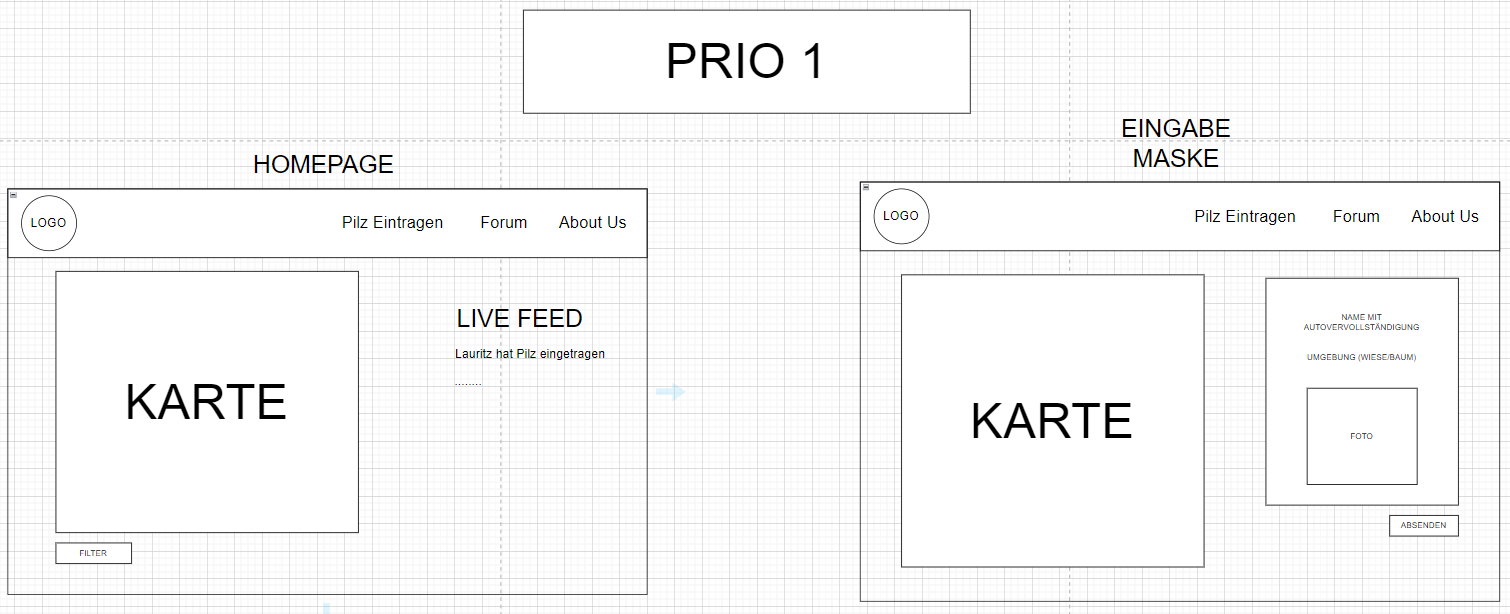
\includegraphics[width=\textwidth]{abbildungen/GuiEntwurfDrawio.jpg}
	\caption{Das Ergebnis des GUI Designs.}
	\label{fig:GUI_Entwurf}
\end{figure}

Nicht-funktionale Anforderungen wie Einfachheit, Benutzerfreundlichkeit und Responsive Design waren hierbei maßgebliche
Faktoren, an denen sich der Designprozess orientierte. Die Einfachheit der Benutzeroberfläche wurde als essenziell erachtet,
um die Nutzerführung intuitiv und zugänglich zu gestalten. So wurde jedes Element der GUI, sowie deren Anordnung, mit dem Ziel
entworfen, eine direkte und unkomplizierte Interaktion möglich zu machen. Benutzerfreundlichkeit stand ebenfalls im Vordergrund,
um sicherzustellen, dass Nutzer aller Erfahrungsstufen die Anwendung problemlos verwenden können. So gibt es keine überflüssigen
Elemente und die vorhandenen sind gut sichtbar und selbsterklärend. Die Anpassung an verschiedene Endgeräte durch ein Responsive
Design war ein weiterer kritischer Aspekt, der ebenfalls Berücksichtigung fand, da die Applikation höhst wahrscheinlich schon
während des Pilzesuchens verwendet wird. So wurde sich entschieden, bei schmaleren Bildschirmen die Karte anstatt auf der linken
Hälfte auf der oberen Hälfte des Bildschrimes anzuzeigen. Der Live-Feed, bzw. die Eingabemaske rutscht in diesem Fall direkt darunter.
So gewährleistet das Responsive Design, dass `ShroomScout' auf Smartphones gleichermaßen funktionell und ästhetisch ansprechend ist,
wie auf Desktops und Tablets.

\subsubsection{Frontend-Framework Entscheidung}

Nach der Gestaltung der GUI stand letztlich noch die Auswahl eines Frontend-Frameworks an. Ein Frontend-Framework ist eine Sammlung
wiederverwendbarer Designvorlagen und Code-Snippets, die Entwicklern helfen, konsistente und effiziente Benutzeroberflächen zu
erstellen. Diese Frameworks bieten vorgefertigte Komponenten und Werkzeuge, die die Entwicklung beschleunigen und die Einhaltung
von Webstandards erleichtern.

Die Entscheidung fiel recht schnell auf Angular, hauptsächlich aufgrund von bereits vorhandenen Erfahrungen und aufgebautem
Basiswissen mit der Technologie. Obwohl andere Frontend-Frameworks wie React und Vue ebenfalls in Betracht gezogen wurden,
gab die Vertrautheit mit Angular den Ausschlag. React, bekannt für seine Flexibilität und Leistung, und Vue, geschätzt für
seine Einfachheit und leichtes Lernen, wären ebenfalls hervorragende Optionen für die Entwicklung moderner Webanwendungen gewesen.
Die Entscheidung für Angular basierte jedoch auf der spezifischen Projekterfahrung und dem Komfortniveau der Entwickler.

Darüber hinaus lassen sich weitere Vorteile von Angular, bzw. generell eines Frontend-Frameworks finden, welche den Entwicklungsprozess
des Frontends unterstützten:

\begin{itemize}

	\item
	      Angular überzeugt durch eine komponentenbasierte Architektur und dadurch modulare Herangehensweise bei der Entwicklung.
	      Jeder Baustein der Anwendung wird dabei in einer Komponente gekapselt, was Klarheit der Anwendungsstruktur fördert und die
	      Wiederverwendung dieser Komponenten möglich macht.

	\item
	      Die Bereitstellung umfangreicher Bibliotheken von eingebauten Funktionen und Diensten, wie Formularverwaltung, Routing oder
	      ein HTTP-Client, bietet durch die Vereinfachung der Entwicklung signifikante Vorteile.

	\item
	      Die Verwendung von TypeScript, welches JavaScript um starke Typisierung und objektorientierte Programmierkonzepte wie Klassen,
	      Interfaces und Dekoratoren erweitert, ermöglicht eine deutlich verbesserte Entwicklungserfahrung.

	\item
	      Angular ermöglicht durch seine umfangreiche Dokumentation und Community-Unterstützung eine effiziente Problemlösung und
	      Weiterentwicklung. Auch lassen sich dadurch zu den meisten Problemen sehr schnell Lösungen finden, was die Geschwindigkeit der
	      Entwicklung beschleunigt.

\end{itemize}

\end{document}
